\documentclass[ignorenonframetext,]{beamer}
\setbeamertemplate{caption}[numbered]
\setbeamertemplate{caption label separator}{: }
\setbeamercolor{caption name}{fg=normal text.fg}
\beamertemplatenavigationsymbolsempty
\usepackage{lmodern}
\usepackage{amssymb,amsmath}
\usepackage{ifxetex,ifluatex}
\usepackage{fixltx2e} % provides \textsubscript
\ifnum 0\ifxetex 1\fi\ifluatex 1\fi=0 % if pdftex
  \usepackage[T1]{fontenc}
  \usepackage[utf8]{inputenc}
\else % if luatex or xelatex
  \ifxetex
    \usepackage{mathspec}
  \else
    \usepackage{fontspec}
  \fi
  \defaultfontfeatures{Ligatures=TeX,Scale=MatchLowercase}
\fi
% use upquote if available, for straight quotes in verbatim environments
\IfFileExists{upquote.sty}{\usepackage{upquote}}{}
% use microtype if available
\IfFileExists{microtype.sty}{%
\usepackage{microtype}
\UseMicrotypeSet[protrusion]{basicmath} % disable protrusion for tt fonts
}{}
\newif\ifbibliography
\hypersetup{
            pdftitle={Module 11: Linear Regression, the g-prior, and model selection},
            pdfauthor={Rebecca C. Steorts},
            pdfborder={0 0 0},
            breaklinks=true}
\urlstyle{same}  % don't use monospace font for urls
\usepackage{color}
\usepackage{fancyvrb}
\newcommand{\VerbBar}{|}
\newcommand{\VERB}{\Verb[commandchars=\\\{\}]}
\DefineVerbatimEnvironment{Highlighting}{Verbatim}{commandchars=\\\{\}}
% Add ',fontsize=\small' for more characters per line
\usepackage{framed}
\definecolor{shadecolor}{RGB}{248,248,248}
\newenvironment{Shaded}{\begin{snugshade}}{\end{snugshade}}
\newcommand{\KeywordTok}[1]{\textcolor[rgb]{0.13,0.29,0.53}{\textbf{#1}}}
\newcommand{\DataTypeTok}[1]{\textcolor[rgb]{0.13,0.29,0.53}{#1}}
\newcommand{\DecValTok}[1]{\textcolor[rgb]{0.00,0.00,0.81}{#1}}
\newcommand{\BaseNTok}[1]{\textcolor[rgb]{0.00,0.00,0.81}{#1}}
\newcommand{\FloatTok}[1]{\textcolor[rgb]{0.00,0.00,0.81}{#1}}
\newcommand{\ConstantTok}[1]{\textcolor[rgb]{0.00,0.00,0.00}{#1}}
\newcommand{\CharTok}[1]{\textcolor[rgb]{0.31,0.60,0.02}{#1}}
\newcommand{\SpecialCharTok}[1]{\textcolor[rgb]{0.00,0.00,0.00}{#1}}
\newcommand{\StringTok}[1]{\textcolor[rgb]{0.31,0.60,0.02}{#1}}
\newcommand{\VerbatimStringTok}[1]{\textcolor[rgb]{0.31,0.60,0.02}{#1}}
\newcommand{\SpecialStringTok}[1]{\textcolor[rgb]{0.31,0.60,0.02}{#1}}
\newcommand{\ImportTok}[1]{#1}
\newcommand{\CommentTok}[1]{\textcolor[rgb]{0.56,0.35,0.01}{\textit{#1}}}
\newcommand{\DocumentationTok}[1]{\textcolor[rgb]{0.56,0.35,0.01}{\textbf{\textit{#1}}}}
\newcommand{\AnnotationTok}[1]{\textcolor[rgb]{0.56,0.35,0.01}{\textbf{\textit{#1}}}}
\newcommand{\CommentVarTok}[1]{\textcolor[rgb]{0.56,0.35,0.01}{\textbf{\textit{#1}}}}
\newcommand{\OtherTok}[1]{\textcolor[rgb]{0.56,0.35,0.01}{#1}}
\newcommand{\FunctionTok}[1]{\textcolor[rgb]{0.00,0.00,0.00}{#1}}
\newcommand{\VariableTok}[1]{\textcolor[rgb]{0.00,0.00,0.00}{#1}}
\newcommand{\ControlFlowTok}[1]{\textcolor[rgb]{0.13,0.29,0.53}{\textbf{#1}}}
\newcommand{\OperatorTok}[1]{\textcolor[rgb]{0.81,0.36,0.00}{\textbf{#1}}}
\newcommand{\BuiltInTok}[1]{#1}
\newcommand{\ExtensionTok}[1]{#1}
\newcommand{\PreprocessorTok}[1]{\textcolor[rgb]{0.56,0.35,0.01}{\textit{#1}}}
\newcommand{\AttributeTok}[1]{\textcolor[rgb]{0.77,0.63,0.00}{#1}}
\newcommand{\RegionMarkerTok}[1]{#1}
\newcommand{\InformationTok}[1]{\textcolor[rgb]{0.56,0.35,0.01}{\textbf{\textit{#1}}}}
\newcommand{\WarningTok}[1]{\textcolor[rgb]{0.56,0.35,0.01}{\textbf{\textit{#1}}}}
\newcommand{\AlertTok}[1]{\textcolor[rgb]{0.94,0.16,0.16}{#1}}
\newcommand{\ErrorTok}[1]{\textcolor[rgb]{0.64,0.00,0.00}{\textbf{#1}}}
\newcommand{\NormalTok}[1]{#1}

% Prevent slide breaks in the middle of a paragraph:
\widowpenalties 1 10000
\raggedbottom

\AtBeginPart{
  \let\insertpartnumber\relax
  \let\partname\relax
  \frame{\partpage}
}
\AtBeginSection{
  \ifbibliography
  \else
    \let\insertsectionnumber\relax
    \let\sectionname\relax
    \frame{\sectionpage}
  \fi
}
\AtBeginSubsection{
  \let\insertsubsectionnumber\relax
  \let\subsectionname\relax
  \frame{\subsectionpage}
}

\setlength{\parindent}{0pt}
\setlength{\parskip}{6pt plus 2pt minus 1pt}
\setlength{\emergencystretch}{3em}  % prevent overfull lines
\providecommand{\tightlist}{%
  \setlength{\itemsep}{0pt}\setlength{\parskip}{0pt}}
\setcounter{secnumdepth}{0}
% Custom definitions
% To use this customization file, insert the line "% Custom definitions
% To use this customization file, insert the line "% Custom definitions
% To use this customization file, insert the line "% Custom definitions
% To use this customization file, insert the line "\input{custom}" in the header of the tex file.

% Formatting

\tolerance=1000
\usepackage[margin=1in]{geometry}


% Packages

% \usepackage{amssymb,latexsym}
\usepackage{amssymb,amsfonts,amsmath,latexsym,amsthm}
%\usepackage[usenames,dvipsnames]{color}
\usepackage[]{graphicx}
\usepackage[space]{grffile}
\usepackage{mathrsfs}   % fancy math font
% \usepackage[font=small,skip=0pt]{caption}
\usepackage[skip=0pt]{caption}
\usepackage{subcaption}
\usepackage{verbatim}
\usepackage{url}
\usepackage{bm}
\usepackage{dsfont}
\usepackage{extarrows}
\usepackage{multirow}
% \usepackage{wrapfig}
% \usepackage{epstopdf}
\usepackage{rotating}
\usepackage{tikz}
\usetikzlibrary{fit}					% fitting shapes to coordinates
%\usetikzlibrary{backgrounds}	% drawing the background after the foreground


% \usepackage[dvipdfm,colorlinks,citecolor=blue,linkcolor=blue,urlcolor=blue]{hyperref}
\usepackage[colorlinks,citecolor=blue,linkcolor=blue,urlcolor=blue]{hyperref}
%\usepackage{hyperref}
\usepackage[authoryear,round]{natbib}


%  Theorems, etc.

\theoremstyle{plain}
\newtheorem{theorem}{Theorem}[section]
\newtheorem{corollary}[theorem]{Corollary}
\newtheorem{lemma}[theorem]{Lemma}
\newtheorem{proposition}[theorem]{Proposition}
\newtheorem{condition}[theorem]{Condition}
% \newtheorem{conditions}[theorem]{Conditions}

\theoremstyle{definition}
\newtheorem{definition}[theorem]{Definition}
% \newtheorem*{unnumbered-definition}{Definition}
\newtheorem{example}[theorem]{Example}
\theoremstyle{remark}
\newtheorem*{remark}{Remark}
\numberwithin{equation}{section}




% Document-specific shortcuts
\newcommand{\btheta}{{\bm\theta}}
\newcommand{\bbtheta}{{\pmb{\bm\theta}}}

\newcommand{\commentary}[1]{\ifx\showcommentary\undefined\else \emph{#1}\fi}

\newcommand{\term}[1]{\textit{\textbf{#1}}}

% Math shortcuts

% Probability distributions
\DeclareMathOperator*{\Exp}{Exp}
\DeclareMathOperator*{\TExp}{TExp}
\DeclareMathOperator*{\Bernoulli}{Bernoulli}
\DeclareMathOperator*{\Beta}{Beta}
\DeclareMathOperator*{\Ga}{Gamma}
\DeclareMathOperator*{\TGamma}{TGamma}
\DeclareMathOperator*{\Poisson}{Poisson}
\DeclareMathOperator*{\Binomial}{Binomial}
\DeclareMathOperator*{\NormalGamma}{NormalGamma}
\DeclareMathOperator*{\InvGamma}{InvGamma}
\DeclareMathOperator*{\Cauchy}{Cauchy}
\DeclareMathOperator*{\Uniform}{Uniform}
\DeclareMathOperator*{\Gumbel}{Gumbel}
\DeclareMathOperator*{\Pareto}{Pareto}
\DeclareMathOperator*{\Mono}{Mono}
\DeclareMathOperator*{\Geometric}{Geometric}
\DeclareMathOperator*{\Wishart}{Wishart}

% Math operators
\DeclareMathOperator*{\argmin}{arg\,min}
\DeclareMathOperator*{\argmax}{arg\,max}
\DeclareMathOperator*{\Cov}{Cov}
\DeclareMathOperator*{\diag}{diag}
\DeclareMathOperator*{\median}{median}
\DeclareMathOperator*{\Vol}{Vol}

% Math characters
\newcommand{\R}{\mathbb{R}}
\newcommand{\Z}{\mathbb{Z}}
\newcommand{\E}{\mathbb{E}}
\renewcommand{\Pr}{\mathbb{P}}
\newcommand{\I}{\mathds{1}}
\newcommand{\V}{\mathbb{V}}

\newcommand{\A}{\mathcal{A}}
\newcommand{\C}{\mathcal{C}}
\newcommand{\D}{\mathcal{D}}
\newcommand{\Hcal}{\mathcal{H}}
\newcommand{\M}{\mathcal{M}}
\newcommand{\N}{\mathcal{N}}
\newcommand{\X}{\mathcal{X}}
\newcommand{\Zcal}{\mathcal{Z}}
\renewcommand{\P}{\mathcal{P}}

\newcommand{\T}{\mathtt{T}}
\renewcommand{\emptyset}{\varnothing}


% Miscellaneous commands
\newcommand{\iid}{\stackrel{\mathrm{iid}}{\sim}}
\newcommand{\matrixsmall}[1]{\bigl(\begin{smallmatrix}#1\end{smallmatrix} \bigr)}

\newcommand{\items}[1]{\begin{itemize} #1 \end{itemize}}

\newcommand{\todo}[1]{\emph{\textcolor{red}{(#1)}}}

\newcommand{\branch}[4]{
\left\{
	\begin{array}{ll}
		#1  & \mbox{if } #2 \\
		#3 & \mbox{if } #4
	\end{array}
\right.
}

% approximately proportional to
\def\app#1#2{%
  \mathrel{%
    \setbox0=\hbox{$#1\sim$}%
    \setbox2=\hbox{%
      \rlap{\hbox{$#1\propto$}}%
      \lower1.3\ht0\box0%
    }%
    \raise0.25\ht2\box2%
  }%
}
\def\approxprop{\mathpalette\app\relax}

% \newcommand{\approptoinn}[2]{\mathrel{\vcenter{
  % \offinterlineskip\halign{\hfil$##$\cr
    % #1\propto\cr\noalign{\kern2pt}#1\sim\cr\noalign{\kern-2pt}}}}}

% \newcommand{\approxpropto}{\mathpalette\approptoinn\relax}





" in the header of the tex file.

% Formatting

\tolerance=1000
\usepackage[margin=1in]{geometry}


% Packages

% \usepackage{amssymb,latexsym}
\usepackage{amssymb,amsfonts,amsmath,latexsym,amsthm}
%\usepackage[usenames,dvipsnames]{color}
\usepackage[]{graphicx}
\usepackage[space]{grffile}
\usepackage{mathrsfs}   % fancy math font
% \usepackage[font=small,skip=0pt]{caption}
\usepackage[skip=0pt]{caption}
\usepackage{subcaption}
\usepackage{verbatim}
\usepackage{url}
\usepackage{bm}
\usepackage{dsfont}
\usepackage{extarrows}
\usepackage{multirow}
% \usepackage{wrapfig}
% \usepackage{epstopdf}
\usepackage{rotating}
\usepackage{tikz}
\usetikzlibrary{fit}					% fitting shapes to coordinates
%\usetikzlibrary{backgrounds}	% drawing the background after the foreground


% \usepackage[dvipdfm,colorlinks,citecolor=blue,linkcolor=blue,urlcolor=blue]{hyperref}
\usepackage[colorlinks,citecolor=blue,linkcolor=blue,urlcolor=blue]{hyperref}
%\usepackage{hyperref}
\usepackage[authoryear,round]{natbib}


%  Theorems, etc.

\theoremstyle{plain}
\newtheorem{theorem}{Theorem}[section]
\newtheorem{corollary}[theorem]{Corollary}
\newtheorem{lemma}[theorem]{Lemma}
\newtheorem{proposition}[theorem]{Proposition}
\newtheorem{condition}[theorem]{Condition}
% \newtheorem{conditions}[theorem]{Conditions}

\theoremstyle{definition}
\newtheorem{definition}[theorem]{Definition}
% \newtheorem*{unnumbered-definition}{Definition}
\newtheorem{example}[theorem]{Example}
\theoremstyle{remark}
\newtheorem*{remark}{Remark}
\numberwithin{equation}{section}




% Document-specific shortcuts
\newcommand{\btheta}{{\bm\theta}}
\newcommand{\bbtheta}{{\pmb{\bm\theta}}}

\newcommand{\commentary}[1]{\ifx\showcommentary\undefined\else \emph{#1}\fi}

\newcommand{\term}[1]{\textit{\textbf{#1}}}

% Math shortcuts

% Probability distributions
\DeclareMathOperator*{\Exp}{Exp}
\DeclareMathOperator*{\TExp}{TExp}
\DeclareMathOperator*{\Bernoulli}{Bernoulli}
\DeclareMathOperator*{\Beta}{Beta}
\DeclareMathOperator*{\Ga}{Gamma}
\DeclareMathOperator*{\TGamma}{TGamma}
\DeclareMathOperator*{\Poisson}{Poisson}
\DeclareMathOperator*{\Binomial}{Binomial}
\DeclareMathOperator*{\NormalGamma}{NormalGamma}
\DeclareMathOperator*{\InvGamma}{InvGamma}
\DeclareMathOperator*{\Cauchy}{Cauchy}
\DeclareMathOperator*{\Uniform}{Uniform}
\DeclareMathOperator*{\Gumbel}{Gumbel}
\DeclareMathOperator*{\Pareto}{Pareto}
\DeclareMathOperator*{\Mono}{Mono}
\DeclareMathOperator*{\Geometric}{Geometric}
\DeclareMathOperator*{\Wishart}{Wishart}

% Math operators
\DeclareMathOperator*{\argmin}{arg\,min}
\DeclareMathOperator*{\argmax}{arg\,max}
\DeclareMathOperator*{\Cov}{Cov}
\DeclareMathOperator*{\diag}{diag}
\DeclareMathOperator*{\median}{median}
\DeclareMathOperator*{\Vol}{Vol}

% Math characters
\newcommand{\R}{\mathbb{R}}
\newcommand{\Z}{\mathbb{Z}}
\newcommand{\E}{\mathbb{E}}
\renewcommand{\Pr}{\mathbb{P}}
\newcommand{\I}{\mathds{1}}
\newcommand{\V}{\mathbb{V}}

\newcommand{\A}{\mathcal{A}}
\newcommand{\C}{\mathcal{C}}
\newcommand{\D}{\mathcal{D}}
\newcommand{\Hcal}{\mathcal{H}}
\newcommand{\M}{\mathcal{M}}
\newcommand{\N}{\mathcal{N}}
\newcommand{\X}{\mathcal{X}}
\newcommand{\Zcal}{\mathcal{Z}}
\renewcommand{\P}{\mathcal{P}}

\newcommand{\T}{\mathtt{T}}
\renewcommand{\emptyset}{\varnothing}


% Miscellaneous commands
\newcommand{\iid}{\stackrel{\mathrm{iid}}{\sim}}
\newcommand{\matrixsmall}[1]{\bigl(\begin{smallmatrix}#1\end{smallmatrix} \bigr)}

\newcommand{\items}[1]{\begin{itemize} #1 \end{itemize}}

\newcommand{\todo}[1]{\emph{\textcolor{red}{(#1)}}}

\newcommand{\branch}[4]{
\left\{
	\begin{array}{ll}
		#1  & \mbox{if } #2 \\
		#3 & \mbox{if } #4
	\end{array}
\right.
}

% approximately proportional to
\def\app#1#2{%
  \mathrel{%
    \setbox0=\hbox{$#1\sim$}%
    \setbox2=\hbox{%
      \rlap{\hbox{$#1\propto$}}%
      \lower1.3\ht0\box0%
    }%
    \raise0.25\ht2\box2%
  }%
}
\def\approxprop{\mathpalette\app\relax}

% \newcommand{\approptoinn}[2]{\mathrel{\vcenter{
  % \offinterlineskip\halign{\hfil$##$\cr
    % #1\propto\cr\noalign{\kern2pt}#1\sim\cr\noalign{\kern-2pt}}}}}

% \newcommand{\approxpropto}{\mathpalette\approptoinn\relax}





" in the header of the tex file.

% Formatting

\tolerance=1000
\usepackage[margin=1in]{geometry}


% Packages

% \usepackage{amssymb,latexsym}
\usepackage{amssymb,amsfonts,amsmath,latexsym,amsthm}
%\usepackage[usenames,dvipsnames]{color}
\usepackage[]{graphicx}
\usepackage[space]{grffile}
\usepackage{mathrsfs}   % fancy math font
% \usepackage[font=small,skip=0pt]{caption}
\usepackage[skip=0pt]{caption}
\usepackage{subcaption}
\usepackage{verbatim}
\usepackage{url}
\usepackage{bm}
\usepackage{dsfont}
\usepackage{extarrows}
\usepackage{multirow}
% \usepackage{wrapfig}
% \usepackage{epstopdf}
\usepackage{rotating}
\usepackage{tikz}
\usetikzlibrary{fit}					% fitting shapes to coordinates
%\usetikzlibrary{backgrounds}	% drawing the background after the foreground


% \usepackage[dvipdfm,colorlinks,citecolor=blue,linkcolor=blue,urlcolor=blue]{hyperref}
\usepackage[colorlinks,citecolor=blue,linkcolor=blue,urlcolor=blue]{hyperref}
%\usepackage{hyperref}
\usepackage[authoryear,round]{natbib}


%  Theorems, etc.

\theoremstyle{plain}
\newtheorem{theorem}{Theorem}[section]
\newtheorem{corollary}[theorem]{Corollary}
\newtheorem{lemma}[theorem]{Lemma}
\newtheorem{proposition}[theorem]{Proposition}
\newtheorem{condition}[theorem]{Condition}
% \newtheorem{conditions}[theorem]{Conditions}

\theoremstyle{definition}
\newtheorem{definition}[theorem]{Definition}
% \newtheorem*{unnumbered-definition}{Definition}
\newtheorem{example}[theorem]{Example}
\theoremstyle{remark}
\newtheorem*{remark}{Remark}
\numberwithin{equation}{section}




% Document-specific shortcuts
\newcommand{\btheta}{{\bm\theta}}
\newcommand{\bbtheta}{{\pmb{\bm\theta}}}

\newcommand{\commentary}[1]{\ifx\showcommentary\undefined\else \emph{#1}\fi}

\newcommand{\term}[1]{\textit{\textbf{#1}}}

% Math shortcuts

% Probability distributions
\DeclareMathOperator*{\Exp}{Exp}
\DeclareMathOperator*{\TExp}{TExp}
\DeclareMathOperator*{\Bernoulli}{Bernoulli}
\DeclareMathOperator*{\Beta}{Beta}
\DeclareMathOperator*{\Ga}{Gamma}
\DeclareMathOperator*{\TGamma}{TGamma}
\DeclareMathOperator*{\Poisson}{Poisson}
\DeclareMathOperator*{\Binomial}{Binomial}
\DeclareMathOperator*{\NormalGamma}{NormalGamma}
\DeclareMathOperator*{\InvGamma}{InvGamma}
\DeclareMathOperator*{\Cauchy}{Cauchy}
\DeclareMathOperator*{\Uniform}{Uniform}
\DeclareMathOperator*{\Gumbel}{Gumbel}
\DeclareMathOperator*{\Pareto}{Pareto}
\DeclareMathOperator*{\Mono}{Mono}
\DeclareMathOperator*{\Geometric}{Geometric}
\DeclareMathOperator*{\Wishart}{Wishart}

% Math operators
\DeclareMathOperator*{\argmin}{arg\,min}
\DeclareMathOperator*{\argmax}{arg\,max}
\DeclareMathOperator*{\Cov}{Cov}
\DeclareMathOperator*{\diag}{diag}
\DeclareMathOperator*{\median}{median}
\DeclareMathOperator*{\Vol}{Vol}

% Math characters
\newcommand{\R}{\mathbb{R}}
\newcommand{\Z}{\mathbb{Z}}
\newcommand{\E}{\mathbb{E}}
\renewcommand{\Pr}{\mathbb{P}}
\newcommand{\I}{\mathds{1}}
\newcommand{\V}{\mathbb{V}}

\newcommand{\A}{\mathcal{A}}
\newcommand{\C}{\mathcal{C}}
\newcommand{\D}{\mathcal{D}}
\newcommand{\Hcal}{\mathcal{H}}
\newcommand{\M}{\mathcal{M}}
\newcommand{\N}{\mathcal{N}}
\newcommand{\X}{\mathcal{X}}
\newcommand{\Zcal}{\mathcal{Z}}
\renewcommand{\P}{\mathcal{P}}

\newcommand{\T}{\mathtt{T}}
\renewcommand{\emptyset}{\varnothing}


% Miscellaneous commands
\newcommand{\iid}{\stackrel{\mathrm{iid}}{\sim}}
\newcommand{\matrixsmall}[1]{\bigl(\begin{smallmatrix}#1\end{smallmatrix} \bigr)}

\newcommand{\items}[1]{\begin{itemize} #1 \end{itemize}}

\newcommand{\todo}[1]{\emph{\textcolor{red}{(#1)}}}

\newcommand{\branch}[4]{
\left\{
	\begin{array}{ll}
		#1  & \mbox{if } #2 \\
		#3 & \mbox{if } #4
	\end{array}
\right.
}

% approximately proportional to
\def\app#1#2{%
  \mathrel{%
    \setbox0=\hbox{$#1\sim$}%
    \setbox2=\hbox{%
      \rlap{\hbox{$#1\propto$}}%
      \lower1.3\ht0\box0%
    }%
    \raise0.25\ht2\box2%
  }%
}
\def\approxprop{\mathpalette\app\relax}

% \newcommand{\approptoinn}[2]{\mathrel{\vcenter{
  % \offinterlineskip\halign{\hfil$##$\cr
    % #1\propto\cr\noalign{\kern2pt}#1\sim\cr\noalign{\kern-2pt}}}}}

% \newcommand{\approxpropto}{\mathpalette\approptoinn\relax}





" in the header of the tex file.

% Formatting

\setbeamertemplate{navigation symbols}{}
\setbeamertemplate{footline}[page number]


\usepackage{bbm}
% Packages
\usepackage{amssymb,amsfonts,amsmath,latexsym,amsthm}
%\usepackage[usenames,dvipsnames]{color}
%\usepackage[]{graphicx}
%\usepackage[space]{grffile}
\usepackage{mathrsfs} 
 \usepackage{amssymb,latexsym}
\usepackage{amssymb,amsfonts,amsmath,latexsym,amsthm, bm}
%\usepackage[usenames,dvipsnames]{color}
%\usepackage[]{graphicx}
%\usepackage[space]{grffile}
\usepackage{mathrsfs}   % fancy math font
% \usepackage[font=small,skip=0pt]{caption}
%\usepackage[skip=0pt]{caption}
%\usepackage{subcaption}
%\usepackage{verbatim}
%\usepackage{url}
%\usepackage{bm}
\usepackage{dsfont}
\usepackage{multirow}
%\usepackage{extarrows}
%\usepackage{multirow}
%% \usepackage{wrapfig}
%% \usepackage{epstopdf}
%\usepackage{rotating}
%\usepackage{tikz}
%\usetikzlibrary{fit}					% fitting shapes to coordinates
%\usetikzlibrary{backgrounds}	% drawing the background after the foreground


% \usepackage[dvipdfm,colorlinks,citecolor=blue,linkcolor=blue,urlcolor=blue]{hyperref}
%\usepackage[colorlinks,citecolor=blue,linkcolor=blue,urlcolor=blue]{hyperref}
%%\usepackage{hyperref}
%\usepackage[authoryear,round]{natbib}


%  Theorems, etc.

%\theoremstyle{plain}
%\newtheorem{theorem}{Theorem}[section]
%\newtheorem{corollary}[theorem]{Corollary}
%\newtheorem{lemma}[theorem]{Lemma}
%\newtheorem{proposition}[theorem]{Proposition}
%\newtheorem{condition}[theorem]{Condition}
% \newtheorem{conditions}[theorem]{Conditions}

%\theoremstyle{definition}
%\newtheorem{definition}[theorem]{Definition}
%% \newtheorem*{unnumbered-definition}{Definition}
%\newtheorem{example}[theorem]{Example}
%\theoremstyle{remark}
%\newtheorem*{remark}{Remark}
%\numberwithin{equation}{section}

\newcommand{\bz}   {\bm{z}}
\newcommand{\bY}   {\bm{Y}}

\newcommand{\hbeta}   {\hat{\beta}}
\newcommand{\hy}   {\hat{y}}


% Document-specific shortcuts
\newcommand{\btheta}{{\bm\theta}}
\newcommand{\bbtheta}{{\pmb{\bm\theta}}}

\newcommand{\commentary}[1]{\ifx\showcommentary\undefined\else \emph{#1}\fi}

\newcommand{\term}[1]{\textit{\textbf{#1}}}

% Math shortcuts

% Probability distributions
\DeclareMathOperator*{\Exp}{Exp}
\DeclareMathOperator*{\TExp}{TExp}
\DeclareMathOperator*{\Bernoulli}{Bernoulli}
\DeclareMathOperator*{\Beta}{Beta}
\DeclareMathOperator*{\Ga}{Gamma}
\DeclareMathOperator*{\TGamma}{TGamma}
\DeclareMathOperator*{\Poisson}{Poisson}
\DeclareMathOperator*{\Binomial}{Binomial}
\DeclareMathOperator*{\NormalGamma}{NormalGamma}
\DeclareMathOperator*{\InvGamma}{InvGamma}
\DeclareMathOperator*{\Cauchy}{Cauchy}
\DeclareMathOperator*{\Uniform}{Uniform}
\DeclareMathOperator*{\Gumbel}{Gumbel}
\DeclareMathOperator*{\Pareto}{Pareto}
\DeclareMathOperator*{\Mono}{Mono}
\DeclareMathOperator*{\Geometric}{Geometric}
\DeclareMathOperator*{\Wishart}{Wishart}

% Math operators
\DeclareMathOperator*{\argmin}{arg\,min}
\DeclareMathOperator*{\argmax}{arg\,max}
\DeclareMathOperator*{\Cov}{Cov}
\DeclareMathOperator*{\diag}{diag}
\DeclareMathOperator*{\median}{median}
\DeclareMathOperator*{\Vol}{Vol}

% Math characters
\newcommand{\R}{\mathbb{R}}
\newcommand{\Z}{\mathbb{Z}}
\newcommand{\E}{\mathbb{E}}
\renewcommand{\Pr}{\mathbb{P}}
\newcommand{\I}{\mathds{1}}
\newcommand{\V}{\mathbb{V}}
\newcommand{\bbeta}{\bm{\beta}}

\newcommand{\A}{\mathcal{A}}
%\newcommand{\C}{\mathcal{C}}
\newcommand{\D}{\mathcal{D}}
\newcommand{\Hcal}{\mathcal{H}}
\newcommand{\M}{\mathcal{M}}
\newcommand{\N}{\mathcal{N}}
\newcommand{\X}{\mathcal{X}}
\newcommand{\Zcal}{\mathcal{Z}}
\renewcommand{\P}{\mathcal{P}}


\newcommand{\T}{\mathtt{T}}
\renewcommand{\emptyset}{\varnothing}

\newcommand{\bmu}{\bm{\mu}}
\newcommand{\by}   {\bm{y}}
\newcommand{\bX}   {\bm{X}}
\newcommand{\sig}   {\Sigma}
\newcommand{\bx}{\ensuremath{\mathbf{x}}}
%\newcommand{\X}{\ensuremath{\mathbf{x}}}
%\newcommand{\w}{\ensuremath{\mathbf{w}}}
%\newcommand{\h}{\ensuremath{\mathbf{h}}}
%\newcommand{\V}{\ensuremath{\mathbf{v}}}
%\newcommand{\cov}{\text{Cov}}
\newcommand{\var}{\text{Var}}
\newcommand{\Var}{\text{Var}}



% Miscellaneous commands
\newcommand{\iid}{\stackrel{\mathrm{iid}}{\sim}}
\newcommand{\matrixsmall}[1]{\bigl(\begin{smallmatrix}#1\end{smallmatrix} \bigr)}

\newcommand{\items}[1]{\begin{itemize} #1 \end{itemize}}

\newcommand{\todo}[1]{\emph{\textcolor{red}{(#1)}}}

\newcommand{\branch}[4]{
\left\{
	\begin{array}{ll}
		#1  & \mbox{if } #2 \\
		#3 & \mbox{if } #4
	\end{array}
\right.
}

% approximately proportional to
\def\app#1#2{%
  \mathrel{%
    \setbox0=\hbox{$#1\sim$}%
    \setbox2=\hbox{%
      \rlap{\hbox{$#1\propto$}}%
      \lower1.3\ht0\box0%
    }%
    \raise0.25\ht2\box2%
  }%
}
\def\approxprop{\mathpalette\app\relax}

% \newcommand{\approptoinn}[2]{\mathrel{\vcenter{
  % \offinterlineskip\halign{\hfil$##$\cr
    % #1\propto\cr\noalign{\kern2pt}#1\sim\cr\noalign{\kern-2pt}}}}}

% \newcommand{\approxpropto}{\mathpalette\approptoinn\relax}

\title{Module 11: Linear Regression, the g-prior, and model selection}
\author{Rebecca C. Steorts}
\date{Hoff, Chapter 9}

\begin{document}
\frame{\titlepage}

\begin{frame}{Agenda}

\begin{itemize}
\tightlist
\item
  Review of the Multivariate setup
\item
  The g-prior
\item
  Application to diabetes (Hoff, 9.2)
\item
  Bayesian model selection (g-prior)
\item
  Bayesian model averaging
\end{itemize}

\end{frame}

\begin{frame}{Notation}

\begin{itemize}
\tightlist
\item
  \(X_{n\times p}\): regression features or covariates (design matrix)
\item
  \(\bx_{p \times 1}\): \(i\)th row vector of the regression covariates
\item
  \(\by_{n\times 1}\): response variable (vector)
\item
  \(\bbeta_{p \times 1}\): vector of regression coefficients
\end{itemize}

\end{frame}

\begin{frame}{Multivariate Setup}

Let's assume that we have data points \((x_i,y_i)\) available for all
\(i=1,\ldots,n.\)

\begin{itemize}
\tightlist
\item
  \(\by\) is the response variable \[  \by= \left( \begin{array}{c}
  y_1\\
  y_2\\
  \vdots\\
  y_n
  \end{array} \right)_{n \times 1} \]
\item
  \(\bx_{i}\) is the \(i\)th row of the design matrix
  \(X_{n \times p}.\)
\end{itemize}

Consider the regression coefficients

\[  \bbeta = \left( \begin{array}{c}
\beta_{1}\\
\beta_{2}\\
\vdots\\
\beta_{p}
\end{array} \right)_{p \times 1} \]

\end{frame}

\begin{frame}{Multivariate Setup}

\[\by \mid X,\bbeta, \sigma^2 \sim MVN( X\bbeta, \sigma^2 I)\]
\[\bbeta \sim MVN(\beta_0, \Sigma_o) \]

Recall the posterior can be shown to be
\[\bbeta \mid \bm{y}, X, \sigma^2 \sim MVN(\bbeta_n, \Sigma_n)\]

where

\[\bbeta_n = E[\bbeta\ \mid \bm{y}, \bX, \sigma^2] = (\Sigma_o^{-1} + (X^TX)^{-1}/\sigma^2)^{-1}
(\Sigma_o^{-1}\bbeta_0 + \bX^T\bm{y}/\sigma^2)\]

\[\Sigma_n = \text{Var}[\bbeta \mid \bm{y}, \bX, \sigma^2] = (\Sigma_o^{-1} + (X^TX)^{-1}/\sigma^2)^{-1}\]
How do we specify \textcolor{red}{a prior on} \(\bbeta_0\) and
\(\Sigma_o\)?

\end{frame}

\begin{frame}{The g-prior}

To do the \emph{least amount of calculus}, we can put a \emph{g-prior}
on \(\bbeta.\)

The g-prior on \(\bbeta\) has the following form:
\[ \bbeta \mid \bX, \sigma^2  \sim MVN(0, g\; \sigma^2 (\bX^T\bX)^{-1}),\]
where \(g\) is a constant, such as \(g=n.\)

The prior also happens to be invariant and is widely studied for
regression problems (Zellner, 1986).

We will find that

\begin{enumerate}
\def\labelenumi{\arabic{enumi}.}
\tightlist
\item
  g shrinks the coefficients and can prevent overfitting to the data
\item
  if \(g = n\), then as n increases, inference approximates that using
  \(\hat{\beta}_{ols}\)
\end{enumerate}

\end{frame}

\begin{frame}{The g-prior}

Under the g-prior, it follows that

\begin{align}
\bbeta_n &= E[\bbeta\ \mid \bm{y}, \bX, \sigma^2]  \\
&= \left(\frac{X^TX}{g \sigma^2} + \frac{X^TX}{\sigma^2}\right)^{-1} \frac{X^Ty}{\sigma^2} \\
&= \frac{g}{g+1} (X^TX)^{-1} X^Ty
= \frac{g}{g+1} \hat{\beta}_{ols}
\end{align}

\begin{align}
\Sigma_n &= \text{Var}[\bbeta \mid \bm{y}, \bX, \sigma^2] \\
&= \left(\frac{X^TX}{g \sigma^2} + \frac{X^TX}{\sigma^2}\right)^{-1}
=\frac{g}{g+1} \sigma^2 (X^TX)^{-1} \\
&= \frac{g}{g+1} \Var[\hat{\beta}_{ols}]
\end{align}

\end{frame}

\begin{frame}{Variance component \(\sigma^2\)}

What about a prior on \(1/\sigma^2 = \lambda\)

\begin{align}
y &\mid X,\beta, \sigma^2 \sim MVN( X\beta, \sigma^2 I) \\
1/\sigma^2 = \lambda &\sim \Ga(\nu_0/2,\nu_0 \sigma_0^2 /2)
\end{align}

Then the posterior can be shown to be

\[p(\sigma^2 \mid y, X) 
\sim \text{InverseGamma}([\nu_0 + n]/2,[\nu_0 \sigma_0^2 + SSR_g]/2).\]\footnote{This is left as an exercise to be done on your own.}

where \(SSR_g\) is somewhat complicated (see Hoff for details, p.~158).

\end{frame}

\begin{frame}{Variance component \(\sigma^2\)}

The joint distribution can be written as

\[p(\sigma^2, \bbeta \mid y, X) = p(\sigma^2 \mid y, X) \times p(\bbeta \mid y,X, \sigma^2)\]

Goal: simulate \((\sigma^2, \bbeta) \sim p(\sigma^2, \bbeta \mid y, X)\)

Starting value \((\bbeta_0, \sigma^2_0)\)

\begin{enumerate}
\def\labelenumi{\arabic{enumi}.}
\item
  Simulate \[\sigma^2 \sim p(\sigma^2 \mid y, X)\] Give us
  \((\sigma^2_1,\bbeta_0)\)
\item
  Use this updated value of \(\sigma^2_1\) to simulate
  \[\bbeta \sim p(\bbeta \mid y,X, \sigma^2_1)\] Gives us
  \((\sigma^2_1, \bbeta_1)\)\footnote{Here, $\bbeta_1$ should not be confused as the first component of the vector of $\bbeta$ as here we are taking a draw from the Gibbs sampler.}
\end{enumerate}

Run the sampler for \(S\) iterations.

\end{frame}

\begin{frame}{Application to diabetes (Exercise 9.2, part a)}

Suppose we have data on health-related variables of a population of 532
women.

Our goal is to model the conditional distribution of glucose level (glu)
as a linear combination of the other variables, excluding the variable
diabetes.\footnote{See Exercise 7.6 for the data description.}

\end{frame}

\begin{frame}{Model specification}

\begin{align}
y &\mid X,\beta, \sigma^2 \sim MVN( X\beta, \lambda^{-1} I) \\
\bbeta &\mid \lambda \sim MVN(0, g \textcolor{red}{\lambda^{-1}} (X^TX)^{-1})\\
\lambda &\sim \Ga(\nu_0/2,\nu_0 \textcolor{red}{\sigma_o^2}/2)
\end{align}

\end{frame}

\begin{frame}{Regression model on the g-prior}

Fit a regression model using the g-prior with g = n, \(\nu_0 = 2\) and
\(\sigma_0^2 = 1.\) Obtain posterior confidence intervals for all of the
parameters.

\end{frame}

\begin{frame}{Regression model on the g-prior}

Section 9.2.2 (Hoff) shows that under the \(g\) prior,
\(p(\sigma^{2}\mid\boldsymbol{y},\boldsymbol{X})\) and
\(p(\boldsymbol{\beta}\mid\boldsymbol{y},\boldsymbol{X},\sigma^{2})\)
are inverse gamma and multivariate normal distributions respectively.

\end{frame}

\begin{frame}{Regression model on the g-prior}

Therefore samples from the joint posterior
\(p(\sigma^{2},\boldsymbol{\beta}\mid\boldsymbol{y},\boldsymbol{X},\sigma^{2})\)
can be made with a Monte Carlo approximation.

We first center and scale all the variables so that there is no need to
include an intercept in the model.

\end{frame}

\begin{frame}[fragile]{Regression model on the g-prior}

\begin{Shaded}
\begin{Highlighting}[]
\CommentTok{#library(knitr)}
\CommentTok{#rm(list=ls())}
\NormalTok{azd_data =}\StringTok{ }\KeywordTok{read.table}\NormalTok{(}\StringTok{"azdiabetes.dat"}\NormalTok{, }\DataTypeTok{header =} \OtherTok{TRUE}\NormalTok{)}
\KeywordTok{head}\NormalTok{(azd_data)}
\end{Highlighting}
\end{Shaded}

\begin{verbatim}
##   npreg glu bp skin  bmi   ped age diabetes
## 1     5  86 68   28 30.2 0.364  24       No
## 2     7 195 70   33 25.1 0.163  55      Yes
## 3     5  77 82   41 35.8 0.156  35       No
## 4     0 165 76   43 47.9 0.259  26       No
## 5     0 107 60   25 26.4 0.133  23       No
## 6     5  97 76   27 35.6 0.378  52      Yes
\end{verbatim}

\end{frame}

\begin{frame}[fragile]{Regression model on the g-prior}

\begin{Shaded}
\begin{Highlighting}[]
\NormalTok{y =}\StringTok{ }\NormalTok{azd_data}\OperatorTok{$}\NormalTok{glu}
\CommentTok{# remove glu and diabetes}
\NormalTok{X =}\StringTok{ }\KeywordTok{as.matrix}\NormalTok{(azd_data[,}\KeywordTok{c}\NormalTok{(}\OperatorTok{-}\DecValTok{2}\NormalTok{,}\OperatorTok{-}\DecValTok{8}\NormalTok{)])}
\KeywordTok{head}\NormalTok{(X)}
\end{Highlighting}
\end{Shaded}

\begin{verbatim}
##      npreg bp skin  bmi   ped age
## [1,]     5 68   28 30.2 0.364  24
## [2,]     7 70   33 25.1 0.163  55
## [3,]     5 82   41 35.8 0.156  35
## [4,]     0 76   43 47.9 0.259  26
## [5,]     0 60   25 26.4 0.133  23
## [6,]     5 76   27 35.6 0.378  52
\end{verbatim}

\end{frame}

\begin{frame}[fragile]{Standardization}

\begin{Shaded}
\begin{Highlighting}[]
\CommentTok{# standardize data to have mean 0 and variance 1}
\NormalTok{ys =}\StringTok{ }\KeywordTok{scale}\NormalTok{(y)}
\NormalTok{Xs =}\StringTok{ }\KeywordTok{scale}\NormalTok{(X)}
\NormalTok{n =}\StringTok{ }\KeywordTok{dim}\NormalTok{(Xs)[}\DecValTok{1}\NormalTok{]}
\NormalTok{p =}\StringTok{ }\KeywordTok{dim}\NormalTok{(Xs)[}\DecValTok{2}\NormalTok{]}
\end{Highlighting}
\end{Shaded}

\end{frame}

\begin{frame}[fragile]{Hyper-parameters}

\begin{Shaded}
\begin{Highlighting}[]
\NormalTok{g =}\StringTok{ }\NormalTok{n}
\NormalTok{nu0 =}\StringTok{ }\DecValTok{2}
\NormalTok{s20 =}\StringTok{ }\DecValTok{1}
\end{Highlighting}
\end{Shaded}

\end{frame}

\begin{frame}[fragile]{Intermediate Matrices}

\begin{Shaded}
\begin{Highlighting}[]
\CommentTok{# intermediate matrices}
\NormalTok{Hg =}\StringTok{ }\NormalTok{(g}\OperatorTok{/}\NormalTok{(g}\OperatorTok{+}\DecValTok{1}\NormalTok{)) }\OperatorTok{*}\StringTok{ }\NormalTok{Xs }\OperatorTok\StringTok{ }\KeywordTok{solve}\NormalTok{(}\KeywordTok{t}\NormalTok{(Xs) }\OperatorTok\StringTok{ }\NormalTok{Xs) }\OperatorTok\StringTok{ }\KeywordTok{t}\NormalTok{(Xs)}
\NormalTok{SSRg =}\StringTok{ }\KeywordTok{t}\NormalTok{(ys) }\OperatorTok\StringTok{ }\NormalTok{( }\KeywordTok{diag}\NormalTok{(}\DecValTok{1}\NormalTok{,}\DataTypeTok{nrow=}\NormalTok{n) }\OperatorTok{-}\StringTok{ }\NormalTok{Hg ) }\OperatorTok\StringTok{ }\NormalTok{ys}
\end{Highlighting}
\end{Shaded}

\end{frame}

\begin{frame}[fragile]{Monte carlo}

\begin{Shaded}
\begin{Highlighting}[]
\CommentTok{# number of posterior samples}
\NormalTok{S =}\StringTok{ }\DecValTok{1000}

\CommentTok{# generate posteriors}
\CommentTok{# we know that the sigma2 is}
\CommentTok{# an updated inverse gamma}
\NormalTok{s2 =}\StringTok{ }\DecValTok{1}\OperatorTok{/}\KeywordTok{rgamma}\NormalTok{(S, (nu0}\OperatorTok{+}\NormalTok{n)}\OperatorTok{/}\DecValTok{2}\NormalTok{, (nu0}\OperatorTok{*}\NormalTok{s20 }\OperatorTok{+}\StringTok{ }\NormalTok{SSRg)}\OperatorTok{/}\DecValTok{2}\NormalTok{)}
\KeywordTok{head}\NormalTok{(s2)}
\end{Highlighting}
\end{Shaded}

\begin{verbatim}
## [1] 0.8757964 0.8670699 0.8333923 0.8522915 0.8581030 0.8492109
\end{verbatim}

\end{frame}

\begin{frame}[fragile]{Monte carlo}

\begin{Shaded}
\begin{Highlighting}[]
\CommentTok{# updated posterior mean and variance}
\CommentTok{# from using the g-prior (see slide 7)}
\NormalTok{Vb =}\StringTok{ }\NormalTok{g}\OperatorTok{*}\KeywordTok{solve}\NormalTok{(}\KeywordTok{t}\NormalTok{(Xs) }\OperatorTok\StringTok{ }\NormalTok{Xs)}\OperatorTok{/}\NormalTok{(g}\OperatorTok{+}\DecValTok{1}\NormalTok{)}
\NormalTok{Eb =}\StringTok{ }\NormalTok{Vb }\OperatorTok\StringTok{ }\KeywordTok{t}\NormalTok{(Xs) }\OperatorTok\StringTok{ }\NormalTok{ys}
\NormalTok{E =}\StringTok{ }\KeywordTok{matrix}\NormalTok{(}\KeywordTok{rnorm}\NormalTok{(S}\OperatorTok{*}\NormalTok{p, }\DecValTok{0}\NormalTok{, }\KeywordTok{sqrt}\NormalTok{(s2)),S,p)}
\CommentTok{# use cholesky factorization }
\NormalTok{beta_s =}\StringTok{ }\KeywordTok{t}\NormalTok{( }\KeywordTok{t}\NormalTok{(E }\OperatorTok\StringTok{ }\KeywordTok{chol}\NormalTok{(Vb)) }\OperatorTok{+}\StringTok{ }\KeywordTok{c}\NormalTok{(Eb)) }

\CommentTok{# transform coefficients to the original scale}
\NormalTok{sd_X =}\StringTok{ }\KeywordTok{apply}\NormalTok{(X,}\DecValTok{2}\NormalTok{,sd)}
\NormalTok{Beta_a =}\StringTok{ }\KeywordTok{sweep}\NormalTok{(beta_s,}\DecValTok{2}\NormalTok{,sd_X,}\DataTypeTok{FUN =} \StringTok{"/"}\NormalTok{)}
\end{Highlighting}
\end{Shaded}

\end{frame}

\begin{frame}[fragile]{The 95\% posterior confidence intervals}

\footnotesize

\begin{Shaded}
\begin{Highlighting}[]
\CommentTok{# 95% credible interval}
\NormalTok{(}\DataTypeTok{Beta_CIa =} \KeywordTok{apply}\NormalTok{(Beta_a, }\DecValTok{2}\NormalTok{, quantile, }\KeywordTok{c}\NormalTok{(}\FloatTok{0.025}\NormalTok{, }\FloatTok{0.975}\NormalTok{)))}
\end{Highlighting}
\end{Shaded}

\begin{verbatim}
##             npreg            bp         skin         bmi       ped
## 2.5%  -0.05269071 -0.0002984302 -0.002941644 0.004704214 0.1080635
## 97.5%  0.01234342  0.0144919397  0.016274524 0.036106047 0.5562314
##              age
## 2.5%  0.01467044
## 97.5% 0.03460817
\end{verbatim}

\begin{Shaded}
\begin{Highlighting}[]
\CommentTok{#kable(data.frame(Beta_CIa))}
\end{Highlighting}
\end{Shaded}

\end{frame}

\begin{frame}{Model selection}

\begin{itemize}
\item Often we have a large number of covariates.
\item Using all of them induces poor statistical performance.
\item How can we reduce the covariates and have good inference and prediction?
\item Common method: Backwards and stepwise regression (slow). 
\end{itemize}

\end{frame}

\begin{frame}{Model selection}

Suppose that we believe some of the regression coefficients are 0.
\vskip 1em Come up with a prior distribution that reflects the
probability of this occuring. \vskip 1em Consider
\[y_i = z_1 b_1 x_{i,1} +\ldots  z_p b_p x_{i,p}, \] where \(b_p\) is a
real number and \(z_j\) indicate which regression coefficients are
nonzero. \vskip 1em Note: \(\beta_j = b_j \times z_j.\)

\end{frame}

\begin{frame}{Bayesian model selection}

Bayesian model selection works by obtaining a posterior distribution for
\(\bz.\) \vskip 1em Assume a prior \(p(\bz)\). \vskip 1em Then
\[p(\bz \mid \bY, \bX) = \frac{p(\bz) p(\bY\mid \bX, \bz)}{\sum_z p(\bz) p(\bY\mid \bX, \bz)}\]

\end{frame}

\begin{frame}{Bayesian model selection}

Suppose we want to compare two models \(z_a\) and \(z_b\) . Consider
\[\text{odds}(z_a,z_b\mid \bY, \bX) = \frac{p(z_a\mid \bY, \bX)}{p(z_b\mid \bY, \bX)}
= \frac{p(z_a)}{p(z_b)} \times \frac{p(\bY\mid \bX, z_a)}{p(\bY\mid \bX, z_b)}\]

This is posterior odds = prior odds \(\times\) ``Bayes factor"

\vskip 1em

``Bayes factor``: how much do the data favor model \(z_a\) over model
\(z_b\)

\vskip 1em

To obtain a posterior distribution over models, we must compute
\(p(\bY \mid \bX, \bz)\) for \emph{each} model under consideration.

\end{frame}

\begin{frame}{Bayesian model selection}

We must compute

\begin{align}
p(y \mid X, \bz) &= \int \int p(y, \bbeta, \sigma^2, \mid X, \bz) \; d\bbeta\; d\sigma^2 \\
&\propto\int \int p(y \mid X, \bz)p(\bbeta \mid X, \bz) p(\sigma^2) \; d\bbeta\; d\sigma^2.
\end{align}

To do the \emph{least amount of calculus}, we can put a \emph{g-prior}
on \(\bbeta\)

\[ \bbeta \mid X, \bz \sim MVN(0, g\; \sigma^2 (X_z^TX_z)^{-1}).\]

\end{frame}

\begin{frame}{Back to the g-prior}

Given the g-prior
\[ \bbeta \mid X, \bz \sim MVN(0, g\; \sigma^2 (X_z^TX_z)^{-1}),\]
\(p(y \mid X, \bz)\) can be worked out in closed form (details p.~165).
\vskip 1em Go through the details on your own.

\end{frame}

\begin{frame}{Back to the g-prior}

This results in being able to compute

\begin{align}
\frac{p(y \mid X, \bz_a) }{p(y \mid X, \bz_b) }
& =
(1 + n)^{(p_{z_b} - p_{z_a})/2}
\times \left( \frac{
s_{z_a}^2}{s_{z_b}^2 } \right)^{1/2}\\
&\times
\left(\frac{s_{z_b}^2 + SSR_{g}^{{z_b}}
}
{s_{z_a}^2 + SSR_{g}^{{z_a}}}
\right)^{(n+1)/2}
\end{align}

We have a ratio of the marginal probabilities, giving us a balance
between model complexity and model fit. \vskip 1em Suppose \(p_{z_b}\)
is large compared to \(p_{z_a}.\) \vskip 1em This causes a penalization
of model \(z_b\) \vskip 1em Note that a large value of
\textcolor{red}{$SSR_{g}^{{z_a}}$ compared with $SSR_{g}^{{z_b}}$ will penalize model $z_a$}.

\end{frame}

\begin{frame}{Bayesian Model Averaging}

Suppose that we have an estimate of \(\bbeta\) from which we can make
predictions.

We may also want a list of relatively high probablitiy models. We can
use a Markov chain to search through the space of models for values of
\(z\) with high posterior probability.

\end{frame}

\begin{frame}{Bayesian model averaging}

Suppose \(p\) is large. Then \(2^p\) models to consider. \vskip 1em
Instead let's use a Gibbs sampler to search through the space of models
for values where \(\bz\) has a high posterior probability. \vskip 1em
Generate a new value of \(\bz\) via \[p(z_j \mid \bY, \bX, \bz_{-j}).\]
\vskip 1em The full conditional that \(z_j=1\) can be written as
\(o_j/(o_j +1).\)

\begin{align}
o_j &= \frac{ p(z_j = 1 \mid \bY, \bX, \bz_{-j})}
{p(z_j = 0 \mid \bY, \bX, \bz_{-j})} \\
&=
\frac{ p(z_j = 1 ) p(\bY \mid \bX, \bz_{-j}, z_j=1) }
{p(z_j = 0) p(\bY \mid \bX, \bz_{-j}, z_j=0)}
\end{align}

\end{frame}

\begin{frame}{Bayesian model averaging}

Note: we may also want to obtain posterior samples of \(\bbeta\) and
\(\sigma^2.\) \vskip 1em Using the conditional distributions from
Section 9.2, we can sample from these directly. \vskip 1em The Gibbs
sampling scheme requires using Section 9.2 and 9.3 (covered in lab).

\end{frame}

\begin{frame}{Bayesian model averaging}

\begin{figure}[htbp]
\begin{center}
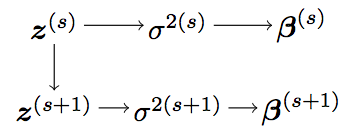
\includegraphics[width=0.4\textwidth]{figures/gibbs-alg}
\caption{Start with $\bz^{(s)}.$ Then in random order update $z_j$ from its full conditional.}
\label{default}
\end{center}
\end{figure}

\end{frame}

\begin{frame}{Bayesian model averaging}

Generate \[\{ \bz^{(s+1)}, \sigma^{2(s+1)}, \bbeta^{(s+1)} \}:\]

\begin{enumerate}
\item Set $\bz = \bz^{(s)}$
\item For $j \in \{1,\ldots, p\}$ in random order, replace $z_j$ with a sample from 
$$p(z_j \mid \bz_{-j}, \bY, \bX)$$
\item Set $\bz^{(s+1)} = \bz^{(s)}$
\item Sample $\sigma^{2(s)} \sim p(\sigma^2 \mid \bz^{(s+1)}, \bY, \bX)$
\item Sample $\bbeta^{(s+1)} \sim p(\bbeta \mid \bz^{(s+1)}, \sigma^{2(s+1)}, \bY, \bX)$
\end{enumerate}

\end{frame}

\begin{frame}{Back to diabetes data (Exercise 9.2, b)}

Let's perform Bayesian model averaging (as described in Section 9.3)

Obtain \(P(\beta_j \neq 0 \mid y)\) as well as posterior confidence
intervals for all of the parameters. Compare our results to that in part
(a.)

\end{frame}

\begin{frame}[fragile]{Back to diabetes data (Exercise 9.2, b)}

The following function \texttt{lpy.X} calculates the log of
\(p(\boldsymbol{y}\mid\boldsymbol{X})\), which we will use in
implementing the Gibbs sampler for Bayesian model averaging.
\footnotesize

\begin{Shaded}
\begin{Highlighting}[]
\NormalTok{## a function to compute the marginal probability}
\NormalTok{lpy.X <-}\StringTok{ }\ControlFlowTok{function}\NormalTok{(y, X, }\DataTypeTok{g=}\KeywordTok{length}\NormalTok{(y), }\DataTypeTok{nu0=}\DecValTok{1}\NormalTok{, }
                  \DataTypeTok{s20=}\KeywordTok{try}\NormalTok{(}\KeywordTok{summary}\NormalTok{(}\KeywordTok{lm}\NormalTok{(y}\OperatorTok{~}\StringTok{ }\OperatorTok{-}\DecValTok{1}\OperatorTok{+}\NormalTok{X))}\OperatorTok{$}\NormalTok{sigma}\OperatorTok{^}\DecValTok{2}\NormalTok{, }\DataTypeTok{silent=}\OtherTok{TRUE}\NormalTok{))\{}
\NormalTok{  n =}\StringTok{ }\KeywordTok{dim}\NormalTok{(X)[}\DecValTok{1}\NormalTok{]}
\NormalTok{  p =}\StringTok{ }\KeywordTok{dim}\NormalTok{(X)[}\DecValTok{2}\NormalTok{]}
  \ControlFlowTok{if}\NormalTok{ (p}\OperatorTok{==}\DecValTok{0}\NormalTok{) \{ Hg =}\StringTok{ }\DecValTok{0}\NormalTok{; s20 =}\StringTok{ }\KeywordTok{mean}\NormalTok{(y}\OperatorTok{^}\DecValTok{2}\NormalTok{)\}}
  \ControlFlowTok{if}\NormalTok{ (p}\OperatorTok{>}\DecValTok{0}\NormalTok{)\{ Hg =}\StringTok{ }\NormalTok{(g}\OperatorTok{/}\NormalTok{(g}\OperatorTok{+}\DecValTok{1}\NormalTok{)) }\OperatorTok{*}\StringTok{ }\NormalTok{X }\OperatorTok\StringTok{ }\KeywordTok{solve}\NormalTok{(}\KeywordTok{t}\NormalTok{(X) }\OperatorTok\StringTok{ }\NormalTok{X) }\OperatorTok\StringTok{ }\KeywordTok{t}\NormalTok{(X) \}}
\NormalTok{  SSRg =}\StringTok{ }\KeywordTok{t}\NormalTok{(y) }\OperatorTok\StringTok{ }\NormalTok{( }\KeywordTok{diag}\NormalTok{(}\DecValTok{1}\NormalTok{, }\DataTypeTok{nrow=}\NormalTok{n) }\OperatorTok{-}\StringTok{ }\NormalTok{Hg ) }\OperatorTok\StringTok{ }\NormalTok{y }\OperatorTok{-}
\StringTok{    }\NormalTok{.}\DecValTok{5}\OperatorTok{*}\NormalTok{( n}\OperatorTok{*}\KeywordTok{log}\NormalTok{(pi) }\OperatorTok{+}\StringTok{ }\NormalTok{p}\OperatorTok{*}\KeywordTok{log}\NormalTok{(}\DecValTok{1}\OperatorTok{+}\NormalTok{g) }\OperatorTok{+}\StringTok{ }\NormalTok{(nu0}\OperatorTok{+}\NormalTok{n)}\OperatorTok{*}\KeywordTok{log}\NormalTok{(nu0}\OperatorTok{*}\NormalTok{s20 }\OperatorTok{+}\StringTok{ }\NormalTok{SSRg) }\OperatorTok{-}\StringTok{ }
\StringTok{           }\NormalTok{nu0}\OperatorTok{*}\KeywordTok{log}\NormalTok{(nu0}\OperatorTok{*}\NormalTok{s20)) }\OperatorTok{+}
\StringTok{    }\KeywordTok{lgamma}\NormalTok{( (nu0}\OperatorTok{+}\NormalTok{n)}\OperatorTok{/}\DecValTok{2}\NormalTok{ ) }\OperatorTok{-}\StringTok{ }\KeywordTok{lgamma}\NormalTok{(nu0}\OperatorTok{/}\DecValTok{2}\NormalTok{)}
\NormalTok{\}}
\end{Highlighting}
\end{Shaded}

\end{frame}

\begin{frame}{Back to diabetes data (Exercise 9.2, b)}

Let \(\boldsymbol{z}\) be the random binary vector of variable
indicators. Generating samples of
\(p(\boldsymbol{z},\sigma^{2},\boldsymbol{\beta})\) from the joint
posterior distribution is achieved with the following steps:

\begin{enumerate}
\def\labelenumi{\arabic{enumi}.}
\item
  For \(j\in\{1,\dots,p\}\) in random order, draw \(z_j\) from
  \(p(z_{j}\mid\boldsymbol{z}_{-j},\boldsymbol{y},\boldsymbol{X})\).
\item
  Sample
  \(\sigma^2 \sim p(\sigma^2 \mid \boldsymbol{z},\boldsymbol{y},\boldsymbol{X})\).
\item
  Sample
  \(\boldsymbol{\beta} \sim p(\boldsymbol{\beta} \mid \boldsymbol{z}, \sigma^2, \boldsymbol{y}, \boldsymbol{X})\).
\end{enumerate}

\end{frame}

\begin{frame}[fragile]{MCMC setup}

\begin{Shaded}
\begin{Highlighting}[]
\NormalTok{g =}\StringTok{ }\NormalTok{n}
\NormalTok{nu0 =}\StringTok{ }\DecValTok{1} \CommentTok{# unit information prior}
\NormalTok{z =}\StringTok{ }\KeywordTok{rep}\NormalTok{(}\DecValTok{1}\NormalTok{, p)}
\CommentTok{# picking a starting value for the marginal probability}
\NormalTok{lpy.c =}\StringTok{ }\KeywordTok{lpy.X}\NormalTok{(ys, Xs[,z}\OperatorTok{==}\DecValTok{1}\NormalTok{,}\DataTypeTok{drop=}\OtherTok{FALSE}\NormalTok{])}
\NormalTok{S =}\StringTok{ }\DecValTok{10}
\NormalTok{Z =}\StringTok{ }\KeywordTok{matrix}\NormalTok{(}\OtherTok{NA}\NormalTok{, S, p)}
\NormalTok{B =}\StringTok{ }\KeywordTok{matrix}\NormalTok{(}\DecValTok{0}\NormalTok{, S, p)}
\end{Highlighting}
\end{Shaded}

\end{frame}

\begin{frame}[fragile]{Gibbs sampler}

\tiny

\begin{Shaded}
\begin{Highlighting}[]
\NormalTok{## Gibbs sampler}
\ControlFlowTok{for}\NormalTok{(s }\ControlFlowTok{in} \DecValTok{1}\OperatorTok{:}\NormalTok{S)\{}
  \CommentTok{# if(s %% 100 ==0) \{print(s)\}}
  \CommentTok{# sample z}
  \ControlFlowTok{for}\NormalTok{ (j }\ControlFlowTok{in} \KeywordTok{sample}\NormalTok{(}\DecValTok{1}\OperatorTok{:}\NormalTok{p))\{}
\NormalTok{    zp =}\StringTok{ }\NormalTok{z}
\NormalTok{    zp[j] =}\StringTok{ }\DecValTok{1} \OperatorTok{-}\StringTok{ }\NormalTok{zp[j]}
\NormalTok{    lpy.p =}\StringTok{ }\KeywordTok{lpy.X}\NormalTok{(ys,Xs[, zp}\OperatorTok{==}\DecValTok{1}\NormalTok{, }\DataTypeTok{drop=}\OtherTok{FALSE}\NormalTok{])}
\NormalTok{    r =}\StringTok{ }\NormalTok{(lpy.p }\OperatorTok{-}\StringTok{ }\NormalTok{lpy.c) }\OperatorTok{*}\StringTok{ }\NormalTok{(}\OperatorTok{-}\DecValTok{1}\NormalTok{)}\OperatorTok{^}\NormalTok{(zp[j]}\OperatorTok{==}\DecValTok{0}\NormalTok{)}
\NormalTok{    zp[j] =}\StringTok{ }\KeywordTok{rbinom}\NormalTok{(}\DecValTok{1}\NormalTok{, }\DecValTok{1}\NormalTok{, }\DecValTok{1}\OperatorTok{/}\NormalTok{(}\DecValTok{1}\OperatorTok{+}\KeywordTok{exp}\NormalTok{(}\OperatorTok{-}\NormalTok{r)))}
    \ControlFlowTok{if}\NormalTok{(z[j] }\OperatorTok{==}\StringTok{ }\NormalTok{zp[j]) \{lpy.c =}\StringTok{ }\NormalTok{lpy.p\}}
\NormalTok{  \}}
\NormalTok{  Z[s,] =}\StringTok{ }\NormalTok{z}
  
  \CommentTok{# sample s2}
\NormalTok{  pm =}\StringTok{ }\KeywordTok{sum}\NormalTok{(z}\OperatorTok{==}\DecValTok{1}\NormalTok{) }\CommentTok{# number of nonzero variables in the model}
  \ControlFlowTok{if}\NormalTok{ (pm}\OperatorTok{==}\DecValTok{0}\NormalTok{)\{ }
\NormalTok{    Hg =}\StringTok{ }\DecValTok{0}
\NormalTok{    s20 =}\StringTok{ }\KeywordTok{mean}\NormalTok{(y}\OperatorTok{^}\DecValTok{2}\NormalTok{)}
\NormalTok{  \}}
  \ControlFlowTok{if}\NormalTok{ (pm}\OperatorTok{>}\DecValTok{0}\NormalTok{)\{}
\NormalTok{    Hg =}\StringTok{ }\NormalTok{(g}\OperatorTok{/}\NormalTok{(g}\OperatorTok{+}\DecValTok{1}\NormalTok{)) }\OperatorTok{*}\StringTok{ }\NormalTok{Xs[,z}\OperatorTok{==}\DecValTok{1}\NormalTok{,drop=F] }\OperatorTok\StringTok{ }\KeywordTok{solve}\NormalTok{(}\KeywordTok{t}\NormalTok{(Xs[,z}\OperatorTok{==}\DecValTok{1}\NormalTok{,}\DataTypeTok{drop=}\NormalTok{F]) }\OperatorTok\StringTok{ }
\StringTok{      }\NormalTok{Xs[,z}\OperatorTok{==}\DecValTok{1}\NormalTok{,}\DataTypeTok{drop=}\NormalTok{F]) }\OperatorTok\StringTok{ }\KeywordTok{t}\NormalTok{(Xs[,z}\OperatorTok{==}\DecValTok{1}\NormalTok{,}\DataTypeTok{drop=}\NormalTok{F])}
    \CommentTok{# estimated residual variance from OLS}
\NormalTok{    s20=}\KeywordTok{summary}\NormalTok{(}\KeywordTok{lm}\NormalTok{(ys }\OperatorTok{~}\StringTok{ }\OperatorTok{-}\DecValTok{1}\OperatorTok{+}\NormalTok{Xs[,z}\OperatorTok{==}\DecValTok{1}\NormalTok{,}\DataTypeTok{drop=}\NormalTok{F]))}\OperatorTok{$}\NormalTok{sigma}\OperatorTok{^}\DecValTok{2}\NormalTok{                                     \}}
  
\NormalTok{  SSRg =}\StringTok{ }\KeywordTok{t}\NormalTok{(ys) }\OperatorTok\StringTok{ }\NormalTok{( }\KeywordTok{diag}\NormalTok{(}\DecValTok{1}\NormalTok{,}\DataTypeTok{nrow=}\NormalTok{n) }\OperatorTok{-}\StringTok{ }\NormalTok{Hg ) }\OperatorTok\StringTok{ }\NormalTok{ys}
\NormalTok{  s2 =}\StringTok{ }\DecValTok{1}\OperatorTok{/}\KeywordTok{rgamma}\NormalTok{(}\DecValTok{1}\NormalTok{, (nu0}\OperatorTok{+}\NormalTok{n)}\OperatorTok{/}\DecValTok{2}\NormalTok{, (nu0}\OperatorTok{*}\NormalTok{s20 }\OperatorTok{+}\StringTok{ }\NormalTok{SSRg)}\OperatorTok{/}\DecValTok{2}\NormalTok{)}
  \CommentTok{# Sigma2[s] = s2}
  
  \CommentTok{# sample beta }
\NormalTok{  Vb =}\StringTok{ }\NormalTok{g }\OperatorTok{*}\StringTok{ }\KeywordTok{solve}\NormalTok{(}\KeywordTok{t}\NormalTok{(Xs[,z}\OperatorTok{==}\DecValTok{1}\NormalTok{,}\DataTypeTok{drop=}\NormalTok{F]) }\OperatorTok\StringTok{ }\NormalTok{Xs[,z}\OperatorTok{==}\DecValTok{1}\NormalTok{,}\DataTypeTok{drop=}\NormalTok{F])}\OperatorTok{/}\NormalTok{(g}\OperatorTok{+}\DecValTok{1}\NormalTok{)}
\NormalTok{  Eb =}\StringTok{ }\NormalTok{Vb }\OperatorTok\StringTok{ }\KeywordTok{t}\NormalTok{(Xs[,z}\OperatorTok{==}\DecValTok{1}\NormalTok{,}\DataTypeTok{drop=}\NormalTok{F]) }\OperatorTok\StringTok{ }\NormalTok{ys}
  
\NormalTok{  E =}\StringTok{ }\KeywordTok{rnorm}\NormalTok{(p, }\DecValTok{0}\NormalTok{, }\KeywordTok{sqrt}\NormalTok{(s2))}
\NormalTok{  beta_z =}\StringTok{ }\NormalTok{E }\OperatorTok\StringTok{ }\KeywordTok{chol}\NormalTok{(Vb) }\OperatorTok{+}\StringTok{ }\KeywordTok{c}\NormalTok{(Eb)}
\NormalTok{  B[s,z}\OperatorTok{==}\DecValTok{1}\NormalTok{] =}\StringTok{ }\NormalTok{beta_z}
\NormalTok{\}}
\end{Highlighting}
\end{Shaded}

\end{frame}

\begin{frame}[fragile]{Results}

The posterior probability
\(\mbox{Pr}(\beta_j \neq 0 \mid \boldsymbol{y})\) is listed below for
each predictor. Clearly all predictors are highly relevant to the
response.

\tiny

\begin{Shaded}
\begin{Highlighting}[]
\NormalTok{pprob_Z =}\StringTok{ }\KeywordTok{apply}\NormalTok{(Z,}\DecValTok{2}\NormalTok{,mean)}
\NormalTok{pprob_Z =}\StringTok{ }\KeywordTok{data.frame}\NormalTok{(}\KeywordTok{matrix}\NormalTok{(pprob_Z,}\DataTypeTok{nr=}\DecValTok{1}\NormalTok{,}\DataTypeTok{nc=}\NormalTok{p))}
\KeywordTok{names}\NormalTok{(pprob_Z) =}\StringTok{ }\KeywordTok{names}\NormalTok{(azd_data[}\KeywordTok{c}\NormalTok{(}\OperatorTok{-}\DecValTok{2}\NormalTok{,}\OperatorTok{-}\DecValTok{8}\NormalTok{)])}
\KeywordTok{row.names}\NormalTok{(pprob_Z) =}\StringTok{ 'posterior including probability'}

\NormalTok{pprob_Z}
\end{Highlighting}
\end{Shaded}

\begin{verbatim}
##                                 npreg bp skin bmi ped age
## posterior including probability     1  1    1   1   1   1
\end{verbatim}

\begin{Shaded}
\begin{Highlighting}[]
\CommentTok{#kable(pprob_Z)}
\end{Highlighting}
\end{Shaded}

\end{frame}

\begin{frame}[fragile]{Results}

The 95\% posterior confidence intervals for all the parameters from
Bayesian model averaging are listed below. The results are similar to
those in part (a) because all the predictors are included in each
iteration of Gibbs sampler all the time.

\footnotesize

\begin{Shaded}
\begin{Highlighting}[]
\CommentTok{# transform coefficients to the original scale}
\CommentTok{#sd_X = apply(X,2,sd)}
\NormalTok{Beta_b =}\StringTok{ }\KeywordTok{sweep}\NormalTok{(B,}\DecValTok{2}\NormalTok{,sd_X,}\DataTypeTok{FUN =} \StringTok{"/"}\NormalTok{)}

\CommentTok{# 95% credible interval}
\NormalTok{(}\DataTypeTok{Beta_CIb =} \KeywordTok{apply}\NormalTok{(Beta_b, }\DecValTok{2}\NormalTok{, quantile, }\KeywordTok{c}\NormalTok{(}\FloatTok{0.025}\NormalTok{, }\FloatTok{0.975}\NormalTok{)))}
\end{Highlighting}
\end{Shaded}

\begin{verbatim}
##               [,1]        [,2]        [,3]        [,4]      [,5]
## 2.5%  -0.046783559 0.003124393 0.001945646 0.008172701 0.2445281
## 97.5%  0.008861632 0.012332815 0.012511617 0.027131571 0.4482633
##             [,6]
## 2.5%  0.01229628
## 97.5% 0.03405374
\end{verbatim}

\end{frame}

\begin{frame}{Preparation for Final Exam}

\begin{itemize}
\tightlist
\item
  April 29, 9 am -- noon, Old Chem 116 PM
\item
  Closed note, closed book
\item
  No calculators
\end{itemize}

\end{frame}

\begin{frame}{Material}

\begin{itemize}
\tightlist
\item
  The exam will be cumulative
\item
  There will be an emphasis on what we covered after Exam II
\item
  You must take the final exam to pass the course
\item
  No make up exams will be given
\end{itemize}

\end{frame}

\begin{frame}{Material after Exam II}

(Modules 8 -- 11)

\begin{itemize}
\tightlist
\item
  Gibbs sampling
\item
  Data augmentation (latent variable models)
\item
  Data augmentation with an application to censored values
\item
  Gaussian mixture models (with latent variables)
\item
  Entity resolution lecture (more latent variable modeling)
\item
  Multivariate distributions and multivariate modeling
\item
  Missing data
\item
  Linear regression
\item
  The g-prior
\item
  Model selection
\end{itemize}

You have many practice exercises posted on this material and the
cumulative material with solutions.

\end{frame}

\begin{frame}{Schedule Before Final Exam}

\begin{itemize}
\tightlist
\item
  Thursday, April 16th: Special lecture by Neil Marchant on how latent
  variables models are used for entity resolution.
\item
  Tuesday, April 23: Prof.~Steorts will hold class at the usual time in
  case there are questions that students wish to go over with me
  relating to the final exam material.
\item
  Wednesday, April 24: Labs will be an extra OH.
\item
  All regular OH by TAs and Professor Steorts will be held through
  Sunday April 28th.
\item
  If you're looking for an old exam, please see Prof.~Steorts after
  class this Thursday or next week in OH.
\item
  Prof Steorts will be happy to give anyone their current class ranking
  after homeworks are calculated next week in OH or near the end of
  class.
\end{itemize}

\end{frame}

\begin{frame}{Resources for the Final Exam}

\begin{itemize}
\tightlist
\item
  There are many practice problems I recommend that are lab exercises.
  \url{https://github.com/resteorts/modern-bayes/tree/master/labs}
\item
  There are many practice exercises that I have posted here to help
  prepare you for the final exam.
  \url{https://github.com/resteorts/modern-bayes/tree/master/exercises}
\end{itemize}

\end{frame}

\end{document}
